\documentclass[a4paper,11pt,titlepage]{article}

\usepackage[utf8]{inputenc}
\usepackage[T1]{fontenc}
\usepackage[english]{babel}
\usepackage{color}
\usepackage{xcolor}
\usepackage{graphicx}
\usepackage{amsmath}
\usepackage{amssymb}
\usepackage{mathtools}
\usepackage{stmaryrd}
\usepackage[hmargin={2.5cm,2.5cm},top=2.5cm,bottom=2.5cm]{geometry}
\usepackage{lmodern}
\usepackage[ruled,lined]{algorithm2e}
\usepackage{listings}
\usepackage{tikz, pgf}

\usepackage[colorlinks=true,breaklinks=true,linkcolor=blue,filecolor=magenta,urlcolor=cyan,pdftitle={Regular Expression Matcher},pdfsubject={Formal Languages}]{hyperref}

\usetikzlibrary{arrows,shapes,positioning}

\title{\underline{Project 1}: Regular Expression Matcher\\\;\\Formal Languages}
\author{HAUTEFAYE Corentin}

\begin{document}

\SetKwComment{Comment}{/* }{ */}
\SetKwInput{Entree}{Input}
\SetKwInput{Sortie}{Output}
\SetKw{KwA}{from}
\SetKw{KwD}{to}
\SetKw{KwO}{OR}
\SetKw{KwE}{AND}
\SetKw{KwN}{NOT}
\SetKwBlock{Deb}{Begin}{End}
\SetKwIF{Si}{SinonSi}{Sinon}{If}{Then}{Else\:if}{Else}{End\:If}
\SetKwFor{Pour}{For}{Do}{End\:For}
\SetKwFor{Tq}{While}{Do}{End\:While}
\SetKwRepeat{Rep}{Repeat}{Until}
\SetKwProg{Fn}{Function}{\\Begin}{End}
\SetKwProg{Pc}{Procedure}{\\Begin}{End}

\maketitle
\newpage

\tableofcontents
\newpage
% ---------------------------------------------------------
\section{Introduction}

\subsection{Problem Statement}
Within the scope of this class on \textit{Formal Languages}, the first assignment I had to work on was to implement a regular expression matcher in Java, C or Python. The goal of this project was to understand how such a program works without using any kind of extern library.

Our program must take two strings as parameters, in other words one for the regular expression and another for the word to check. At the end, this has to return whether such word is spanned by that regular expression or not. This program should handle basic operations on regular expressions ; the latter is described in the following subsection.

\subsection{Notations}
Let $r$ and $s$ be two regular expressions. Then, we have the following:
\begin{itemize}
    \item $r$ and $s$ are called \textit{atomic expressions}.
    \item $(r)$ is a regular expression.
    \item $rs$ denotes the \textit{concatenation} of $r$ and $s$.
    \item $r|s$\footnote{Please see section \ref{sec_alter}} denotes an \textit{alternative} (or union) between $r$ and $s$.
    \item $r*$ denotes the \textit{transitive closure} of $r$.
    \item $r+$ denotes the \textit{positive closure} of $r$.
    \item $r?$ denotes a \textit{choice} to put $r$ or not. 
\end{itemize}
\;\\
From those operators, we can draw the following properties:
\begin{itemize} \label{sec_properties}
    \item $r+=rr*$.
    \item $r?=r|\epsilon$.
    \item A single character has the highest precedence.
    \item Closure (such as *, + or ?) has a lower precedence than a character.
    \item Concatenation has a lower precedence than closure.
    \item Union has a lower precedence than concatenation.
    \item Union has the lowest precedence.
    \item Grouping regular expressions with parenthesis overrides precedence.
\end{itemize}

% ---------------------------------------------------------
\section{Algorithms \& Implementation}
\subsection{Choices}
I have chosen to implement this project in C99 as I am much more comfortable in using that language. Moreover, I only needed structures and not classes to program, thus the choice was quite quick.

\pagebreak
\label{sec_alter}
I have also decided to replace the notation used in the instructions for union (\textit{i.e for all $r$ and $s$ two regular expressions, $r+s$ was replaced by $r|s$}) for several reasons. First of all, I did not like the idea of having the same character '+' used for different purposes as building the syntax tree would have been more difficult. Then, that rule implied that even writing a very simple regular expression using an operator with two different precedences could lead to difficulties and could be ambiguous. For instance, let $r, s$ and $t$ be three regular expressions. The following $r+s+t$ is not entirely clear, except if we put parenthesis but this operation is costly to write and to parse (\textit{especially for top-down recursive algorithms}). Thus, we could interpret it as $(r+s+t)$, $(r+)(s+)(t+)$, $(r+)(s+(t)+)$ and so on... Whereas, $r|s|t$ is not ambiguous at all.

The design of this project can be described in three steps. First, we need to parse a regular expression so that it can be read properly by the program afterwards. I decided to parse it into an abstract syntax tree. Then, I had several choices I could make to use that tree. Thus, I decided to reproduce what I would have done, that is turn the previous tree into an automaton. Once that step is done, matching the given word is pretty easy as the program just has to follow each state in the automaton so that it would arrive in an accepting state or not.

Finally, this project has been compiled on Windows with CLion. It should be able to compile also on any Linux distribution with GCC installed.

\subsection{Parser}

Let $\mathcal{A}$ be a finite set of characters that we will call alphabet. Using the properties in section \ref{sec_properties}, we can formally define a grammar $G=(\mathcal{A}\cup\{(,),|,*,+,?\},\{X,C,R,A\},\to,X)$ such that we have the following axioms : $\left\{\begin{array}{ll}
    X &\to C\;('|'\;C)^*\\
    C&\to R^+\\
    R&\to A\;('*'\;|\;\;'+'\;|\;'?')^*\\
    A&\to \;'('X')'\;|\;c\in\mathcal{A}
\end{array}\right.$ where characters between simple quotes are terminal.

It is now easy to write a parser that follows these rules. However, we do need a structure to hold the data parsed by this automaton. Therefore, we will use an abstract syntax tree defined as follows: $\verb|Node| : \left\{\begin{array}{ll}
    \verb|type| &:\verb|unsigned integer|\\
    \verb|value| &:\verb|character|\\
    \verb|left| &:\verb|Node|\\
    \verb|right| &:\verb|Node|
\end{array}\right.$. 

Furthermore, we assume that a node can have one of the following types:
\begin{itemize}
    \item Character
    \item Concatenation
    \item Union
    \item Star (\textit{transitive closure})
    \item Star (\textit{transitive closure})
    \item Optional (\textit{choice})
\end{itemize}

% ---------------------------------------------------------
\subsection{Non-Deterministic Finite Automaton}
We use the same notations as in the previous subsection. For any abstract syntax tree, it is possible to create a non-deterministic finite automaton step by step. This can be proven with a mathematical induction.

Thus, we need to define trivial cases as well as induction cases. Let $q$ be the initial state and $f$ be the final state.

\subsubsection*{Trivial cases} For the empty word $\epsilon$, we have:
\begin{center}
    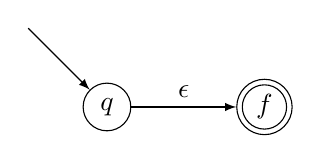
\begin{tikzpicture}
        \node[draw, circle] (q) at (-1,0) {$q$} ;
        \node[draw, circle] (f) at (1,0) {$f$} ;
        \draw[draw, inner sep=1pt]  (1,0) circle (8pt);
        
        \draw[->,>=latex] (q) -- (f) node[above,midway] {$\epsilon$};
        \draw[->,>=latex] (-2,1) -- (q);

    \end{tikzpicture}
\end{center}
\;\\
\\
Let $c\in\mathcal{A}$. For the regular expression $c$, we have:
\begin{center}
    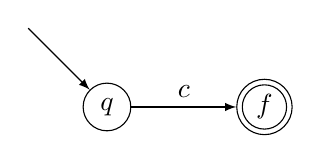
\begin{tikzpicture}
        \node[draw, circle] (q) at (-1,0) {$q$} ;
        \node[draw, circle] (f) at (1,0) {$f$} ;
        \draw[draw, inner sep=1pt]  (1,0) circle (8pt);
        
        \draw[->,>=latex] (q) -- (f) node[above,midway] {$c$};
        \draw[->,>=latex] (-2,1) -- (q);

    \end{tikzpicture}
\end{center}

\subsubsection*{Induction} Let $r$ and $s$ be two regular expressions. Without loss of generality, we denote an automaton of $r$ by $N(r)$.
\;\\\\
For the regular expression $rs$, we put $N(r)$ and $N(s)$ right after the other, whence:
\begin{center}
    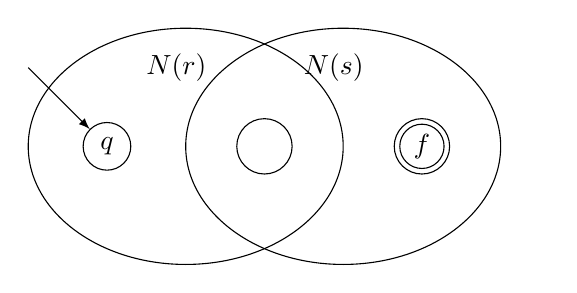
\begin{tikzpicture}
        \node[draw, circle] (q) at (-1,0) {$q$} ;
        \node[draw, circle] (f) at (3,0) {$f$} ;
        \draw[draw, inner sep=1pt]  (3,0) circle (8pt);
        
        \draw[draw, inner sep=1pt]  (1,0) circle (10pt);

        \draw (0,0) ellipse (2cm and 1.5cm);
        \draw (2,0) ellipse (2cm and 1.5cm);

        \node[text width=3cm] at (1,1) {$N(r)$};
        \node[text width=3cm] at (3,1) {$N(s)$};
        
        \draw[->,>=latex] (-2,1) -- (q);

    \end{tikzpicture}
\end{center}

\;\\\\For the regular expression $r|s$, we have two $\epsilon$-transitions towards $N(r)$ and $N(s)$, whence:
\begin{center}
    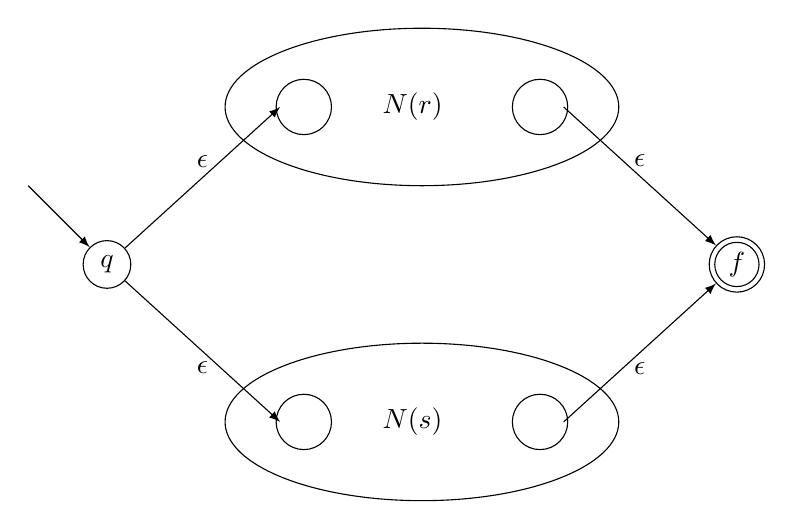
\begin{tikzpicture}
        \node[draw, circle] (q) at (-3,0) {$q$} ;
        \node[draw, circle] (f) at (5,0) {$f$} ;
        \draw[draw, inner sep=1pt]  (5,0) circle (8pt);
        
        \draw[draw, inner sep=1pt]  (-0.5,2) circle (10pt);
        \draw[draw, inner sep=1pt]  (-0.5,-2) circle (10pt);
        \draw[draw, inner sep=1pt]  (2.5,2) circle (10pt);
        \draw[draw, inner sep=1pt]  (2.5,-2) circle (10pt);

        \draw (1,2) ellipse (2.5cm and 1cm);
        \draw (1,-2) ellipse (2.5cm and 1cm);

        \node[text width=3cm] at (2,2) {$N(r)$};
        \node[text width=3cm] at (2,-2) {$N(s)$};
        
        \draw[->,>=latex] (-4,1) -- (q);

        \draw[->,>=latex] (q) -- (-0.8, 2) node[above,midway] {$\epsilon$};
        \draw[->,>=latex] (q) -- (-0.8, -2) node[below,midway] {$\epsilon$};

        \draw[->,>=latex] (2.8, 2) -- (f) node[above,midway] {$\epsilon$};
        \draw[->,>=latex] (2.8, -2) -- (f) node[below,midway] {$\epsilon$};
        
    \end{tikzpicture}
\end{center}

\pagebreak 
\;\\For the regular expression $r^*$, we have:
\begin{center}
    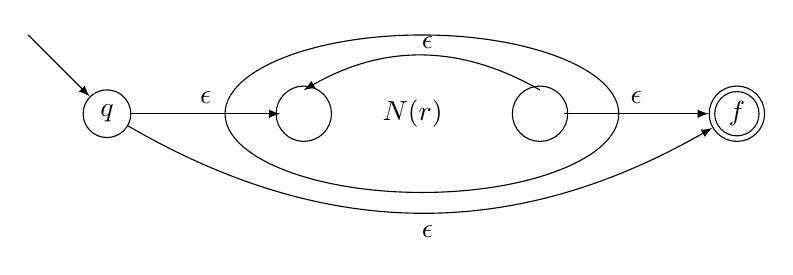
\begin{tikzpicture}
        \node[draw, circle] (q) at (-3,0) {$q$} ;
        \node[draw, circle] (f) at (5,0) {$f$} ;
        \draw[draw, inner sep=1pt]  (5,0) circle (8pt);
        
        \draw[draw, inner sep=1pt]  (-0.5,0) circle (10pt);
        \draw[draw, inner sep=1pt]  (2.5,0) circle (10pt);

        \draw (1,0) ellipse (2.5cm and 1cm);

        \node[text width=3cm] at (2,0) {$N(r)$};
        
        \draw[->,>=latex] (-4,1) -- (q);

        \draw[->,>=latex] (q) -- (-0.8, 0) node[above,midway] {$\epsilon$};
        \draw[->,>=latex] (2.8,0) -- (f) node[above,midway] {$\epsilon$};

        \draw[->,>=latex] (q) edge[bend right] (f) ;
        \node[text width=2cm] at (2,-1.5) {$\epsilon$};

        \draw [->,>=latex] (2.5,0.3) to[bend right](-0.5,0.3);
        \node[text width=2cm] at (2,0.9) {$\epsilon$};
    \end{tikzpicture}
\end{center}

Using the properties in section \ref{sec_properties}, automata for $r^+$ and $r^?$ can be built easily using the previous rules.

Thus these rules yield that an automaton in this context has both starting and accepting states ; the latter are unique. Moreover, a state allows no more than two transitions. By convention, we choose to represent the $\epsilon$-transition by using the null-character, denoted by $\backslash0$ or $0$. If a state does not have $\epsilon$ as a transition, then there is only one transition which is not empty. Thus, we can define the following structures :
$\verb|State| : \left\{\begin{array}{ll}
    \verb|id| &:\verb|unsigned integer|\\
    \verb|transition| &:\verb|character|\\
    \verb|out1| &:\verb|State|\\
    \verb|out2| &:\verb|State|
\end{array}\right.$ and $\verb|Fragment| : \left\{\begin{array}{ll}
    \verb|start| &:\verb|State|\\
    \verb|final| &:\verb|State|
\end{array}\right.$. 

Furthermore, for an easier implementation, we assume that there will be no more than a certain amount of states in our automaton. Here, we have chosen 1024.

% ---------------------------------------------------------
\subsection{Matching}

The algorithm used to match a word with a given non-deterministic finite automaton as defined above is not very complex. However, we do need a structure to hold all states from a given state, so that if a chosen "path" does not succeed, the program can go back and try another state. Thus, we have: $\verb|StateSet| : \left\{\begin{array}{ll}
    \verb|states| &:\verb|array<State>[1024]|\\
    \verb|count| &:\verb|unsigned integer|
\end{array}\right.$. This structure would be equivalent to a stack of which \verb|count| is the top.

\begin{algorithm}[H]
    \caption{Add a state to look at if it has not already been visited}
    \Entree{$E$: StateSet, $Q$: State, $v$: Array<boolean>}
    \Sortie{$\emptyset$}
    \Pc{add\_state(E: StateSet, Q: State, v: Array<boolean>)}{
        \Si{$E\ne\emptyset$ \KwE $Q\ne\emptyset$ \KwE \KwN $v[\text{id}(Q)]$} {
            $v[\text{id}(Q)]\gets\text{True}$\;
            $\left(\text{states}(E)\right)[\text{count}(E)] \gets Q;$\;
            $\text{count}(E)\gets\text{count}(E)+1$\;

            \Si(\Comment*[f]{$\epsilon$-transitions}){$\text{transition}(Q) = \;'\backslash0'$} {
                add\_state($E, \text{out1}(Q), v$)\;
                add\_state($E, \text{out2}(Q), v$)\;
            }
        }
    }
\end{algorithm}

\begin{algorithm}[H]
    \caption{Look at each state from the current state set and try to move to another state}
    \Entree{$Current$: StateSet, $c$: character, $Next$: StateSet}
    \Sortie{$\emptyset$}
    \Pc{step(Current: StateSet, c: character, Next: StateSet)}{
        $\text{count}(Next)\gets0$\;
        $v:\text{Array<boolean>}[1024]\gets\{\text{False}\}$\;
        $i:\text{unsigned integer}\gets0$\;
        $n:\text{unsigned integer}\gets\text{count}(Current)$\;
        \Pour{$i$ \KwA 0 \KwD $n$}{
            $s:\text{State}\gets\text{states}(Current)[i]$\;
            \Si{$\text{transition}(s) = c$ \KwE $\text{out1}(s)\ne\emptyset$} {
                add\_state($Next, \text{out1}(s), v$)\;
            }
        }
    }
\end{algorithm}

\begin{algorithm}[H]
    \caption{Matching a string with a given automaton}
    \Entree{$Q$: State, $F$: State, $S$: string}
    \Sortie{Boolean}
    \Fn{match(Q: State, F: State, S: string) : boolean}{
        $Current:\text{StateSet}$\;
        $Next:\text{StateSet}$\;

        $\text{count}(Current)\gets0$\;
        $v:\text{Array<boolean>}[1024]\gets\{\text{False}\}$\;
        add\_state($Current, Q, v$)\;

        $i:\text{unsigned integer}\gets0$\;
        \Tq{$S[i]\ne \;'\backslash0'$}{
            step($Current, s[i], Next$)\;
            \tcp{Shallow copy}$Current\gets Next$\; 
            $i\gets i+1$\;
        }
        $n:\text{unsigned integer}\gets\text{count}(Current)$\;
        \Pour{$i$ \KwA 0 \KwD $n$}{
            \Si{$\text{states}(Current)[i]=F$} {
                $\text{match}\gets\text{True}$\;
            }
        }
        $\text{match}\gets\text{False}$\;
    }
\end{algorithm}
% ---------------------------------------------------------
\pagebreak
\section{Example}
Let's consider the following regular expression $r=(a|b)^*a$. Thus, here $\mathcal{A}=\{a,b\}$. Let's first build the abstract syntax tree. Using the rules described in section \ref{sec_properties}, we get:
\begin{center}
    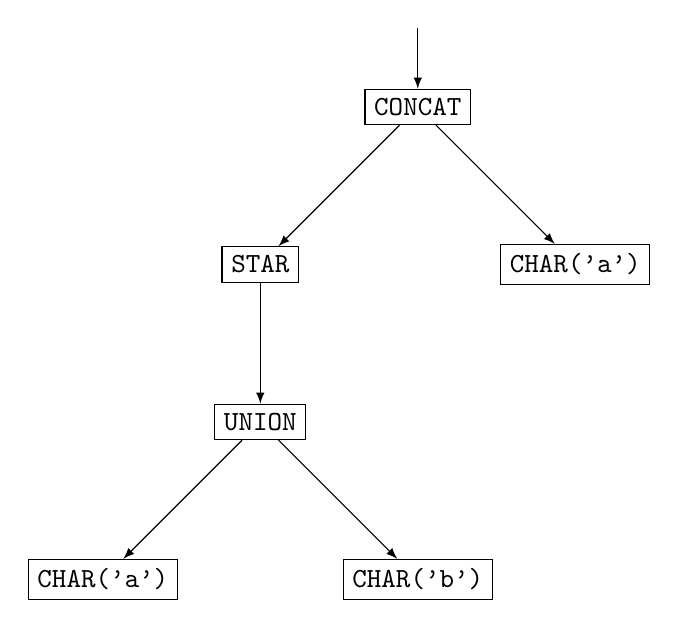
\begin{tikzpicture}
        \node[draw] (A1) at (0,0) {\verb|CONCAT|} ;
        
        \node[draw] (B1) at (-2,-2) {\verb|STAR|} ;
        \node[draw] (B2) at (2,-2) {\verb|CHAR('a')|} ;
        
        \node[draw] (C1) at (-2,-4) {\verb|UNION|} ;
        
        \node[draw] (D1) at (-4,-6) {\verb|CHAR('a')|} ;
        \node[draw] (D2) at (0,-6) {\verb|CHAR('b')|} ;

        \draw[->,>=latex] (0, 1) -- (A1) ;
        \draw[->,>=latex] (A1) -- (B1) ;
        \draw[->,>=latex] (A1) -- (B2) ;
        \draw[->,>=latex] (B1) -- (C1) ;
        \draw[->,>=latex] (C1) -- (D1) ;
        \draw[->,>=latex] (C1) -- (D2) ;
    \end{tikzpicture}
\end{center}

We can construct our non-deterministic finite automaton step by step. We will denote each state by $\left(S_i\right)_{i\in\mathbb{N}}$. First, we have two trivial cases:

\begin{center}
    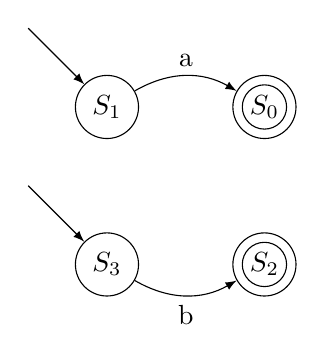
\begin{tikzpicture}
        \node[draw, circle] (S1) at (-1,1) {$S_1$};
        \node[draw, circle] (S0) at (1,1) {$S_0$};
        \draw[draw, inner sep=1pt]  (S0) circle (8pt);
        
        \node[draw, circle] (S3) at (-1,-1) {$S_3$};
        \node[draw, circle] (S2) at (1,-1) {$S_2$};
        \draw[draw, inner sep=1pt]  (S2) circle (8pt);

        \draw[->,>=latex] (-2,2) -- (S1);
        \draw[->,>=latex] (-2,0) -- (S3);

        \draw[->,>=latex] (S1)  to[bend left] node[above]{a} (S0);
        \draw[->,>=latex] (S3)  to[bend right] node[below]{b} (S2);
    \end{tikzpicture}
\end{center}

Afterwards, we have an union of the two previous expressions. Thus, we get:

\begin{center}
    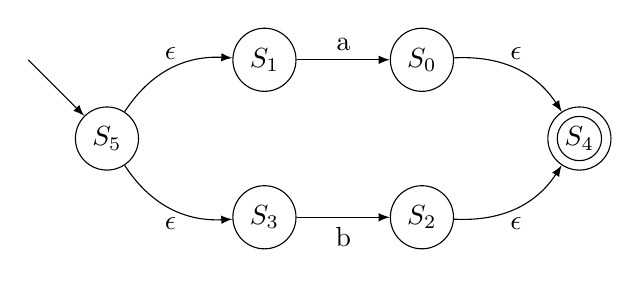
\begin{tikzpicture}
        \node[draw, circle] (S1) at (-1,1) {$S_1$};
        \node[draw, circle] (S0) at (1,1) {$S_0$};
        
        \node[draw, circle] (S3) at (-1,-1) {$S_3$};
        \node[draw, circle] (S2) at (1,-1) {$S_2$};

        \node[draw, circle] (S5) at (-3,0) {$S_5$};
        \node[draw, circle] (S4) at (3,0) {$S_4$};
        \draw[draw, inner sep=1pt]  (S4) circle (8pt);

        \draw[->,>=latex] (-4,1) -- (S5);

        \draw[->,>=latex] (S1)  to node[above]{a} (S0);
        \draw[->,>=latex] (S3)  to node[below]{b} (S2);
        
        \draw[->,>=latex] (S5)  to[bend left] node[above]{$\epsilon$} (S1);
        \draw[->,>=latex] (S0)  to[bend left] node[above]{$\epsilon$} (S4);
        \draw[->,>=latex] (S5)  to[bend right] node[below]{$\epsilon$} (S3);
        \draw[->,>=latex] (S2)  to[bend right] node[below]{$\epsilon$} (S4);
    \end{tikzpicture}
\end{center}
\pagebreak
Then, we need to apply a transitive closure onto the previous automaton. Thus:

\begin{center}
    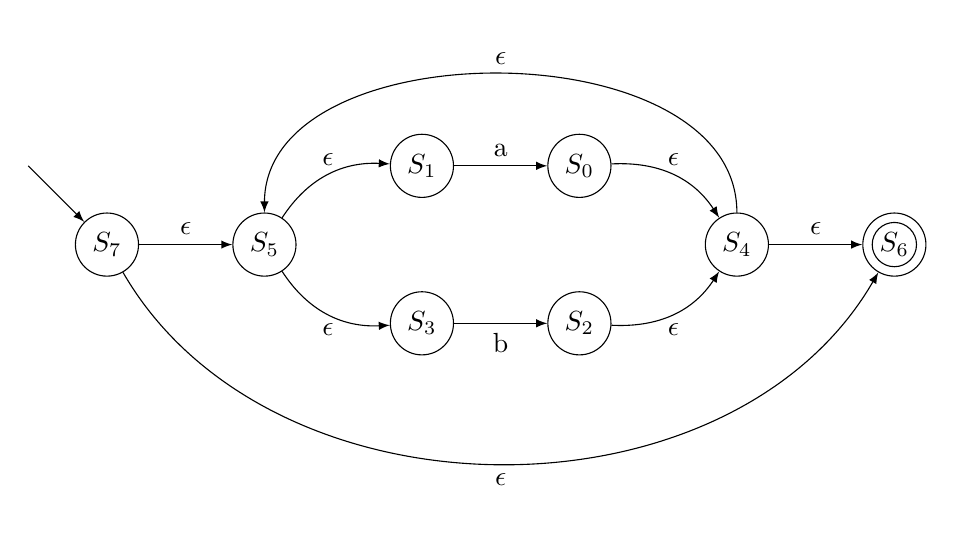
\begin{tikzpicture}
        \node[draw, circle] (S1) at (-1,1) {$S_1$};
        \node[draw, circle] (S0) at (1,1) {$S_0$};
        
        \node[draw, circle] (S3) at (-1,-1) {$S_3$};
        \node[draw, circle] (S2) at (1,-1) {$S_2$};

        \node[draw, circle] (S5) at (-3,0) {$S_5$};
        \node[draw, circle] (S4) at (3,0) {$S_4$};
        
        \node[draw, circle] (S7) at (-5,0) {$S_7$};
        \node[draw, circle] (S6) at (5,0) {$S_6$};
        \draw[draw, inner sep=1pt]  (S6) circle (8pt);

        \draw[->,>=latex] (-6,1) -- (S7);

        \draw[->,>=latex] (S1)  to node[above]{a} (S0);
        \draw[->,>=latex] (S3)  to node[below]{b} (S2);
        
        \draw[->,>=latex] (S7)  to node[above]{$\epsilon$} (S5);
        \draw[->,>=latex] (S4)  to node[above]{$\epsilon$} (S6);
        
        \draw[->,>=latex] (S5)  to[bend left] node[above]{$\epsilon$} (S1);
        \draw[->,>=latex] (S0)  to[bend left] node[above]{$\epsilon$} (S4);
        \draw[->,>=latex] (S5)  to[bend right] node[below]{$\epsilon$} (S3);
        \draw[->,>=latex] (S2)  to[bend right] node[below]{$\epsilon$} (S4);
        
        \draw[->,>=latex] (S4)  to[bend right=90] node[above]{$\epsilon$} (S5);
        \draw[->,>=latex] (S7)  to[bend right=60] node[below]{$\epsilon$} (S6);
    \end{tikzpicture}
\end{center}

Next, we have another atomic expression:
\begin{center}
    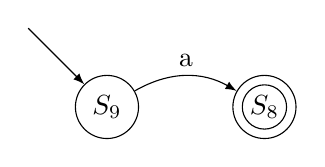
\begin{tikzpicture}
        \node[draw, circle] (S9) at (-1,1) {$S_9$};
        \node[draw, circle] (S8) at (1,1) {$S_8$};
        \draw[draw, inner sep=1pt]  (S8) circle (8pt);

        \draw[->,>=latex] (-2,2) -- (S9);

        \draw[->,>=latex] (S9)  to[bend left] node[above]{a} (S8);
    \end{tikzpicture}
\end{center}

Finally, we need to concatenate the last two automata to get $r$, whence:
\begin{center}
    \begin{tikzpicture}
        \node[draw, circle] (S1) at (-1,1) {$S_1$};
        \node[draw, circle] (S0) at (1,1) {$S_0$};
        
        \node[draw, circle] (S3) at (-1,-1) {$S_3$};
        \node[draw, circle] (S2) at (1,-1) {$S_2$};

        \node[draw, circle] (S5) at (-3,0) {$S_5$};
        \node[draw, circle] (S4) at (3,0) {$S_4$};
        
        \node[draw, circle] (S7) at (-5,0) {$S_7$};
        \node[draw, circle] (S6) at (5,0) {$S_6$};

        \node[draw, circle] (S9) at (7,0) {$S_9$};
        \node[draw, circle] (S8) at (9,0) {$S_8$};
        \draw[draw, inner sep=1pt]  (S8) circle (8pt);

        \draw[->,>=latex] (-6,1) -- (S7);

        \draw[->,>=latex] (S1)  to node[above]{a} (S0);
        \draw[->,>=latex] (S3)  to node[below]{b} (S2);
        
        \draw[->,>=latex] (S7)  to node[above]{$\epsilon$} (S5);
        \draw[->,>=latex] (S4)  to node[above]{$\epsilon$} (S6);
        
        \draw[->,>=latex] (S6)  to node[above]{$\epsilon$} (S9);
        \draw[->,>=latex] (S9)  to node[above]{a} (S8);
        
        \draw[->,>=latex] (S5)  to[bend left] node[above]{$\epsilon$} (S1);
        \draw[->,>=latex] (S0)  to[bend left] node[above]{$\epsilon$} (S4);
        \draw[->,>=latex] (S5)  to[bend right] node[below]{$\epsilon$} (S3);
        \draw[->,>=latex] (S2)  to[bend right] node[below]{$\epsilon$} (S4);
        
        \draw[->,>=latex] (S4)  to[bend right=90] node[above]{$\epsilon$} (S5);
        \draw[->,>=latex] (S7)  to[bend right=60] node[below]{$\epsilon$} (S6);
    \end{tikzpicture}
\end{center}

Let $w_1=aaab$, $w_2=ccabacc$ and $w_3=a$. Let's find whether there exists an accepting configuration for these words.

\paragraph*{Study of $w_1$} Going to $S_6$ does not yield an accepting configuration as we would have $(w_1,S_7)\vdash(w_1, S_6)\vdash(w_1,S_9)\vdash(aab,S_8)\nvdash(\epsilon,S_8)$. Thus, we must have $(w_1,S_7)\vdash(w_1,S_5)$. We can easily apply each transition to get $(\epsilon,S_4)\vdash(\epsilon,S_6)\vdash(\epsilon,S_9)$. However, we cannot go from $S_9$ to $S_8$ as it is not an $\epsilon$-transition. Moreover, all states have been studied. Therefore, \fbox{$w_1$ is not accepted.}

\paragraph*{Study of $w_2$} First, going to $S_5$ is useless since both $S_1$ and $S_3$ do not have a transition for character 'c'. Thus, we have $(w_2,S_7)\vdash(w_2,S_6)\vdash(w_2,S_9)$. Yet, $S_9$ does not have a transition for character 'c'. Since $S_9$ is not terminal, \fbox{$w_2$ is not accepted.}

\paragraph*{Study of $w_3$} Going to state $S_5$ would again lead to $(\epsilon,S_9)$ which is not accepting. Thus, $(w_3,S_7)\vdash(w_3,S_6)\vdash(w_3,S_9)\vdash(\epsilon,S_8)$. Since $S_8$ is final and there is no letter left to proceed, we get that \fbox{$w_3$ is accepted.}
\newline\newline
Let's now try to run the program with $r$ and $w_1$, whence:
\begin{verbatim}
======================
Syntax tree for regex: "(a|b)*a"
----------------------
ROOT
|_ CONCAT
    |- STAR
    |   |_ UNION
    |       |- CHAR('a')
    |       |_ CHAR('b')
    |_ CHAR('a')
======================
Non-Deterministic Finite Automaton:
----------------------
State 7: \0 -> 5, 6
State 6: \0 -> 9
State 9: 'a' -> 8
State 8: \0
State 5: \0 -> 1, 3
State 3: 'b' -> 2
State 2: \0 -> 4
State 4: \0 -> 5, 6
State 1: 'a' -> 0
State 0: \0 -> 4
======================
Matching word "aaab":
----------------------
Current character: 'a'
----------------------
|  Peeking State 7
|  Peeking State 5
|  Peeking State 1
|->Transition State 1 -> State 0
|  Peeking State 3
|  Peeking State 6
|  Peeking State 9
|->Transition State 9 -> State 8
----------------------
Current character: 'a'
----------------------
|  Peeking State 0
|  Peeking State 4
|  Peeking State 5
|  Peeking State 1
|->Transition State 1 -> State 0
|  Peeking State 3
|  Peeking State 6
|  Peeking State 9
|->Transition State 9 -> State 8
|  Peeking State 8
----------------------
Current character: 'a'
----------------------
|  Peeking State 0
|  Peeking State 4
|  Peeking State 5
|  Peeking State 1
|->Transition State 1 -> State 0
|  Peeking State 3
|  Peeking State 6
|  Peeking State 9
|->Transition State 9 -> State 8
|  Peeking State 8
----------------------
Current character: 'b'
----------------------
|  Peeking State 0
|  Peeking State 4
|  Peeking State 5
|  Peeking State 1
|  Peeking State 3
|->Transition State 3 -> State 2
|  Peeking State 6
|  Peeking State 9
|  Peeking State 8
----------------------

Word "aaab" is not accepted!
\end{verbatim}

\underline{N.B}: The procedure \verb|print_tree| first prints the left, then the right nodes for any node in a given tree.

Here, we can see how the previous algorithms processed both the regular expression as well as the word. The final result is correct.
% ---------------------------------------------------------
\section{Feedback}
\subsection{Difficulties}
At first, I had some difficulties because I tried to work only with deterministic finite automata. My functions were indeed very hectic, so I tried another approach. 

I wanted to convert directly the string into a graph ; thus matching the word would have been very easy as we just had to run through the graph. This method worked but did not account for grouping with parenthesis. 

Finally, I had the idea to use an abstract syntax tree, yet I did not know how to turn it into an automaton. So I started to sketch different "fragments" of automata that I could combine to represent a given regular expression. At the end, I realized that those rules were the same seen during the lecture on non-deterministic automata ; that was my clue. From there, I was able to implement everything as intended, except for the notation of the union which I decided to change.

\subsection{Suggestions}
This program is not perfect at all. For instance, I used two global variables whereas it is not recommended in C. The way parameters are passed to the program is not very versatile. For example, I could have chosen to use "short" parameters such as "-r" or "-s", but I did not think at that time that it really mattered. Moreover, as of now, due to the way arguments are passed to a program through the command prompt (\textit{or terminal}), it is not possible to recognize words with whitespace within, unless it is done directly during the execution. Therefore, it may have been better to have a menu with the following choices: 
\begin{enumerate}
    \item Enter regular expression
    \item Match a word
    \item Quit
\end{enumerate}
% ---------------------------------------------------------
\section{Conclusion}
\textit{In fine}, working onto this project was very interesting as I had never tried it before. I was able to define properly objects and properties on the theoretical plane, and to have a concrete application of the latter. The way non-deterministic finite automata are built was both intriguing and fun to understand and to discover by myself.
% ---------------------------------------------------------

\end{document}
